%%
%% This is file `team-eagle-lazer-fang.tex',
%%
%% A modified copy of:
%%
%% sample-authordraft.text
%% 
%% IMPORTANT NOTICE:
%% 
%% For the copyright see the source file.
%% 
%% Any modified versions of this file must be renamed
%% with new filenames distinct from sample-manuscript.tex.
%% 
%% For distribution of the original source see the terms
%% for copying and modification in the file samples.dtx.
%% 
%% This generated file may be distributed as long as the
%% original source files, as listed above, are part of the
%% same distribution. (The sources need not necessarily be
%% in the same archive or directory.)
%%
%% The first command in your LaTeX source must be the \documentclass command.
%%%% Small single column format, used for CIE, CSUR, DTRAP, JACM, JDIQ, JEA, JERIC, JETC, PACMCGIT, TAAS, TACCESS, TACO, TALG, TALLIP (formerly TALIP), TCPS, TDSCI, TEAC, TECS, TELO, THRI, TIIS, TIOT, TISSEC, TIST, TKDD, TMIS, TOCE, TOCHI, TOCL, TOCS, TOCT, TODAES, TODS, TOIS, TOIT, TOMACS, TOMM (formerly TOMCCAP), TOMPECS, TOMS, TOPC, TOPLAS, TOPS, TOS, TOSEM, TOSN, TQC, TRETS, TSAS, TSC, TSLP, TWEB.
% \documentclass[acmsmall]{acmart}

%%%% Large single column format, used for IMWUT, JOCCH, PACMPL, POMACS, TAP, PACMHCI
% \documentclass[acmlarge,screen]{acmart}

%%%% Large double column format, used for TOG
% \documentclass[acmtog, authorversion]{acmart}

%%%% Generic manuscript mode, required for submission
%%%% and peer review
\documentclass[manuscript,screen,review]{acmart}

\usepackage{tikz}
\usetikzlibrary{shapes.geometric, arrows, patterns}
\usepackage{graphicx}
\usepackage{subcaption}
% \usepackage{draftwatermark}
% \SetWatermarkText{\includegraphics[width = 0.25\textwidth, opacity = 0.1]{graphics/Untitled-1.png}}
%% Fonts used in the template cannot be substituted; margin 
%% adjustments are not allowed.
%%
%% \BibTeX command to typeset BibTeX logo in the docs
\AtBeginDocument{%
  \providecommand\BibTeX{{%
    \normalfont B\kern-0.5em{\scshape i\kern-0.25em b}\kern-0.8em\TeX}}}

%% Rights management information.  This information is sent to you
%% when you complete the rights form.  These commands have SAMPLE
%% values in them; it is your responsibility as an author to replace
%% the commands and values with those provided to you when you
%% complete the rights form.
% \setcopyright{acmcopyright}
% \copyrightyear{2018}
% \acmYear{2018}
% \acmDOI{XXXXXXX.XXXXXXX}

% %% These commands are for a PROCEEDINGS abstract or paper.
% \acmConference[Conference acronym 'XX]{Make sure to enter the correct
%   conference title from your rights confirmation emai}{June 03--05,
%   2018}{Woodstock, NY}
% %
% %  Uncomment \acmBooktitle if th title of the proceedings is different
% %  from ``Proceedings of ...''!
% %
% \acmBooktitle{Woodstock '18: ACM Symposium on Neural Gaze Detection,
%  June 03--05, 2018, Woodstock, NY} 
% \acmPrice{15.00}
% \acmISBN{978-1-4503-XXXX-X/18/06}


%%
%% Submission ID.
%% Use this when submitting an article to a sponsored event. You'll
%% receive a unique submission ID from the organizers
%% of the event, and this ID should be used as the parameter to this command.
%%\acmSubmissionID{123-A56-BU3}

%%
%% The majority of ACM publications use numbered citations and
%% references.  The command \citestyle{authoryear} switches to the
%% "author year" style.
%%
%% If you are preparing content for an event
%% sponsored by ACM SIGGRAPH, you must use the "author year" style of
%% citations and references.
%% Uncommenting
%% the next command will enable that style.
%%\citestyle{acmauthoryear}

%%
%% end of the preamble, start of the body of the document source.
\begin{document}

%%
%% The "title" command has an optional parameter,
%% allowing the author to define a "short title" to be used in page headers.
\title{Trustworthiness of AI decision making tools in high-risk applications.}

%%
%% The "author" command and its associated commands are used to define
%% the authors and their affiliations.
%% Of note is the shared affiliation of the first two authors, and the
%% "authornote" and "authornotemark" commands
%% used to denote shared contribution to the research.
\author{Alex Davies}
\affiliation{%
  \institution{Interactive AI CDT, University of Bristol}
  \country{UK}
}
\author{Daniel Collins}
\affiliation{%
  \institution{Interactive AI CDT, University of Bristol}
  \country{UK}
}
\author{Isabella Degen}
\affiliation{%
  \institution{Interactive AI CDT, University of Bristol}
  \country{UK}
}
\author{Jonathan Erskine}
\affiliation{%
  \institution{Interactive AI CDT, University of Bristol}
  \country{UK}
}
\author{Matt Clifford}
\affiliation{%
  \institution{Interactive AI CDT, University of Bristol}
  \country{UK}
}
\author{Ronja Spaniel}
\affiliation{%
  \institution{Interactive AI CDT, University of Bristol}
  \country{UK}
}

%%
%% By default, the full list of authors will be used in the page
%% headers. Often, this list is too long, and will overlap
%% other information printed in the page headers. This command allows
%% the author to define a more concise list
%% of authors' names for this purpose.
\renewcommand{\shortauthors}{Team Eagle Lazer Fang, et al.}

%%
%% The abstract is a short summary of the work to be presented in the
%% article.
\begin{abstract}
Abstract
 Include motivation and Contribution
 what's our contribution - first sentence
 why are we doing this research -> one sentence
 mention survey of x people and focus group -> one sentence on what we did
 what have we done - why is it new - how have we done it - what are our findings (short)
 
 
 
\end{abstract}

%%
%% The code below is generated by the tool at http://dl.acm.org/ccs.cfm.
%% Please copy and paste the code instead of the example below.
%%
% \begin{CCSXML}
% <ccs2012>
%  <concept>
%   <concept_id>10010520.10010553.10010562</concept_id>
%   <concept_desc>Computer systems organization~Embedded systems</concept_desc>
%   <concept_significance>500</concept_significance>
%  </concept>
%  <concept>
%   <concept_id>10010520.10010575.10010755</concept_id>
%   <concept_desc>Computer systems organization~Redundancy</concept_desc>
%   <concept_significance>300</concept_significance>
%  </concept>
%  <concept>
%   <concept_id>10010520.10010553.10010554</concept_id>
%   <concept_desc>Computer systems organization~Robotics</concept_desc>
%   <concept_significance>100</concept_significance>
%  </concept>
%  <concept>
%   <concept_id>10003033.10003083.10003095</concept_id>
%   <concept_desc>Networks~Network reliability</concept_desc>
%   <concept_significance>100</concept_significance>
%  </concept>
% </ccs2012>
% \end{CCSXML}

% \ccsdesc[500]{Computer systems organization~Embedded systems}
% \ccsdesc[300]{Computer systems organization~Redundancy}
% \ccsdesc{Computer systems organization~Robotics}
% \ccsdesc[100]{Networks~Network reliability}

%%
%% Keywords. The author(s) should pick words that accurately describe
%% the work being presented. Separate the keywords with commas.
\keywords{XAI, Explainable AI, Trustworthy AI, Interpretable AI, AI, Computer Automation, AI in high risk}

%%
%% This command processes the author and affiliation and title
%% information and builds the first part of the formatted document.
\maketitle

\newpage
\section{Introduction}\label{sec:introduction}
%%%%%%%%%%%
% Keeping notes from previous list making
%%%%%%%%%%%
%Motivate the research
%give an overview of relevant background literature
%describe the research question.
%Possibly signpost the findings
% notes on how to writing
% go straight to the point
% don't make it so general that it could be used for an other paper
% don't slash others works
% include problem / solution

%Initial structure:
%\begin{itemize}
%    \item AI used in many use applications (give examples of high risk etc) - we focused on healthcare
%    \item For successful integration of AI, users and public need to trust it. 
%    \item Law came into that decisions for banks etc needed to be explained to the user, the right to explanation, e.g GDPR %https://www.turing.ac.uk/research/impact-stories/a-right-to-explanation
%    \item this brought about interest in XAI (Why XAI has been seen as important (Issues with this - black box models, not always human able to intervene/oversee))
%    \item Lots of work has been done into XAI techniques to give `trust' in AI.
%    \item XAI examples to show off the amount of work been done  - survey papers and specific examples? LIME? FATF?
%    \item Issues with XAI - critics (to give some doubt over XAI actually giving trust and telling us how AI works)
%    \item Is the current work in XAI just useful for machine learning practitioners? 
%    \item What is best for the users/ what do users actually want? Has the explanation law confused us of what users actually want/need?
%    \item We want to explore what trust actually is in relation to AI. Is it XAI? Is it performance? Is it counterfactual results? (are they more intuitive/what people would like to know)?
%    \item There has been the topic of trust between humans and machines before (1987 paper). Which indicates that there needs to be trust not just performance.
%    \item There is no current user study of how XAI changes trust depending on: demographic (AI expert, high stakes decision maker, general public) or the level of explainablity. 
%    % \item medical domain - paper Alex found on simple AI in a medical context out-performing doctors
%\end{itemize}
%Ann's suggestion of structure:
%\begin{itemize}
%    \item Context (how is the world now): Messy, AI and Explainable AI, 
%    \item the problem (drama): loads of research, not many survey on what's needed on trust, does transparency and explainable creates more or less trust
%    \item related work and how it doesn't cover this: GDPR has created a flood of research into Explainable AI, so it's not been questioned much on the motivations. Surveys on trust in generic AI systems. Surveys of perspectives on generic AI system for healthcare work groups.
%    \item our solution, method and results: survey and focus group to find out if trust increases with transparency and if experience with AI or high stakes decision making matters
%    \item what new worlds does our research do: design with all demographics in mind, different branches of explainability. Present information that can be used to design better AI systems for healthcare needs. Encourage more user driven explainable AI with the demographics we find
%\end{itemize}

% Isabella: I've kept the bullet points for the text below in my google doc if needed
%%%%%%%%%%%%%%%%


% Why Context - how is the world now
AI is being deployed in a variety of different domains, including high-risk application areas where algorithms are potentially making life-altering decisions; from insurance to criminal justice to healthcare systems \cite{Bohr2020}, \cite{Chen2018}. It is widely believed that new laws like the EU General Data Protection Regulation (GDPR) mandate a ‘right to explanation’ as a mechanism to enhance the accountability and transparency of automated decision-making \cite{Wachter2017}. While that right does not explicitly exist \cite{Wachter2017}, the approval of the GDPR in 2016 created an explosion of research in Explainable AI (XAI) and closely related research areas such as: Transparent AI, Interpretable AI and Trustworthy AI. The desired outcome of these research areas is to create responsible and ethical AI systems that are fair and allow for accountability \cite{Mohseni2021}, often referred to as Responsible AI. This has led to a surge of new methods that explain the decisions of different AI algorithms, see \cite{Linardatos2021} and \cite{Guidotti2018a} for an overview. There are endeavours to standardise and asses explanations \cite{Gilpin2019}; as well as countless literature surveys aiming to create an unified and standardised taxonomy and definitions for explainable, transparent, interpretable and trustworthy AI \cite{Schwalbe2021} and \cite{Arrieta2020}.\\\\

%Why new - The problem (drama)
The huge increase in the popularity of explainable, interpretable and trustworthy AI has given rise to critical views. The motivations behind explainable AI, the quality \cite{Doshi-Velez2017} and usefulness of the explanations given \cite{Miller2019} as well as whether explainable AI achieves its objective of higher trust in AI \cite{Lipton2018} have been studied. Research into explainable AI recognises that there are many different stakeholders of AI systems such as: developers, end-users and lawmakers. The needs of each of these stakeholders vary greatly. For the developers of AI systems the explanations are useful for evaluating, testing and debugging purposes. They have a deep and technical understanding of the concepts and mathematics behind the algorithms and are therefore able to interpret mathematical explanations of those systems. These are the people who are creating new explainability methods and we refer to them as AI experts \cite{Carvalho2019}. The end users of the AI systems are people who use these systems in their work e.g clinicians. They are domain experts in the problem that the AI system solves. These end users are interested in explanations to help them assess the model’s decision and decide on the actions to be taken. Examples of research into how well their needs are served with interpretable and explainable AI can be found in \cite{Goldstein2021}, \cite{Liao2020}, \cite{Salimiparsa2021}. However, there is a lack of research into whether people who are affected by the decisions of an AI system, for example patients that are being diagnosed by an AI system, are asking for more transparent and explainable AI systems.\\\\

%more related work
A study surveyed 922 women’s attitude toward AI in mammography screening. They found that they preferred a combination of radiologist and AI system \cite{Ongena2021}. Another study surveyed 216 fracture patients on their perceptions towards AI used to assist in interpretation of their radiographs and found that participant’s held the clinician’s assessment in the highest regard \cite{York2020}. A further study found that patients are apprehensive about the use of AI \cite{Richardson2021} and highlighted the need for early patient involvement in the AI systems being used in healthcare. These studies did not investigate the role that transparency and performance of the AI system played in the patients attitudes.\\\\

% more related work and how it doesn't cover this: Surveys on trust in generic AI systems. Surveys of perspectives on generic AI systems for healthcare work groups.
There is no current user study of how XAI changes trust depending on: demographic (AI expert, high stakes decision maker, general public) nor the level of explainability.\\  

%What & How: our solution, method and results: survey and focus group to find out if trust increases with transparency and if experience with AI or high stakes decision making matters
In this study we are focusing on the opinions of people who are affected by the decision of an AI system. We created a survey of $n=277$ people who were asked to imagine being diagnosed in a hospital whether to have treatment for COVID or not in four different scenarios:

\begin{enumerate}
    \item A doctor makes the diagnosis.
    \item A doctor makes the diagnosis together with an interpretable AI system (a so called glass box system).
    \item A doctor makes the diagnosis together with an AI system that’s not interpretable (a so called black box system).
    \item A black box system makes the diagnosis by itself.
\end{enumerate}

For each of these scenarios the participants were told how often the doctor and AI system make the correct diagnosis (the performance) and how much the doctor knew about why the AI system made its decision (the interpretability of the system). The participants were asked to express how much they would trust to be diagnosed by that setup by selecting a number from 1-10. We furthermore collected demographic information about the participants, namely if they are working in healthcare or not, how much experience and knowledge they have about AI as well as how frequently they are making high-stakes decisions (life-altering decisions). The scenarios were designed in such a way that the doctor and glass box had the same performance of 85 correct diagnoses out of 100 while the black box had a significantly better performance of 95 correct diagnoses out of 100. We analysed the responses with regards to which scenario was trusted the most respectively least and how this changed depending on the participants demographic. We found that overall scenario 4 (the black box on its own) was the least trusted scenario and scenario 2 (the doctor working together with the glass box) was the most trusted scenario. Scenario 1 (the doctor on their own) surprisingly was the second least trusted scenario, while it was at the same time second most trusted scenario. Scenario 3 (the doctor working with the black box) gained significantly more trust than scenario 4 (the black box on its own). The three demographic aspects did not change this other than for the participants that reported making frequent high stakes decisions, they gave the doctor by themselves the least trust. Furthermore, participants with medium and high AI expertise trust scenario 3 (the doctor with the black box) more. Participants who work in healthcare either trust the doctor by itself a lot or not at all, while participants who don’t work in healthcare trust the black box by itself significantly less.

We followed the survey up with a focus group of 6 people with demographics <?> to discuss and reflect further on their thoughts about AI and the need for interpretability and explanations as well as exploring if black box models will ever be accepted. We found that the dislike of the black box has less to do with the lack of interpretablity, but more to do with the lack of empathy that a machine can give compared to a human when diagnosing someone with a potential critical illness. However, the focus group rated the black box higher than the survey participant did under the conditions that it had high performance and that the patient had full disclosure of a black box being used or that it was used in a low-stakes application area.


%Why relevant: what new worlds does our research do: design with all demographics in mind, different branches of explainability. Present information that can be used to design better AI systems for healthcare needs. Encourage more user driven explainable AI with the demographics we find
<todo> We believe that for an AI system to be adapted in a critical decision scenario, such as diagnosis in health care, it is not sufficient to just make the system transparent and explainable. It is far more important to complete the user experience and give an understanding that the AI system is only a part of that experience. We believe that more research is needed to understand this area fully.\\
The current techniques are useful for the operators of the systems, however, the law is to protect the end user that is affected by an AI having been used. It is clear that the needs for these groups are different and more research needs to be done to consider the end users of those systems and what their needs are and how they differ from the operators.\\


\section{Related Work}
Literature Review

Rough overview
\begin{itemize}
    \item critics of XAI - is it what we really need for trust?, does it really given an explanation for a non AI expert? 
    \item trustworthiness? does XAI make us trust? Lipton paper (Mythos) is trustworthiness resolved XAI or is it performance?
\end{itemize}

\subsection{Available Techniques for Explainability and Interpretability}
There has been a previous wave of explainability in control systems as well as AI in the late 80ies: Explaining Control Strategies in Problem Solving\cite{Chandrasekaran1989}

There's been a plethora of interpretability and explainability techniques developed in recent years - surge since 2016. There are many survey papers that describe the different techniques and try to come up with a framework to organise them:
\begin{itemize}
    \item Explainable AI: A Review of Machine Learning Interpretability Methods\cite{Linardatos2021}
    \item Notions of explainability and evaluation approaches for explainable artificial intelligence\cite{Vilone2021}
    \item A Comprehensive Taxonomy for Explainable Artificial Intelligence: A Systematic Survey of Surveys on Methods and Concepts\cite{Schwalbe2021}
    \item Explainable Artificial Intelligence: a Systematic Review\cite{Vilone2020}
    \item A Survey of Methods for Explaining Black Box Models\cite{Guidotti2018a}
    \item Peeking Inside the Black-Box: A Survey on Explainable Artificial Intelligence (XAI)\cite{Adadi2018}
    \item A Multidisciplinary Survey and Framework for Design and Evaluation of Explainable AI Systems\cite{Mohseni2021}
    \item Explainable Deep Learning: A Field Guide for the Uninitiated\cite{Ras2020}
    \item How Case-Based Reasoning Explains Neural Networks: A Theoretical Analysis of XAI Using Post-Hoc Explanation-by-Example from a Survey of ANN-CBR Twin-Systems\cite{Keane2019}
    \item Improving fairness in machine learning systems: What do industry practitioners need?\cite{Holstein2019}
    \item Good Counterfactuals and Where to Find Them: A Case-Based Technique for Generating Counterfactuals for Explainable AI (XAI)\cite{Keane2020} 
    \item Contrastive explanation: A structural-model approach\cite{Miller2021}
\end{itemize}

\subsection{Papers that argue the need of XAI}
\begin{itemize}
    \item XAI-Explainable artificial intelligence\cite{Gunning2019} Quote "Explainability is essential for users to effectively understand, trust, and manage powerful artificial intelligence applications."
\end{itemize}


\subsection{Shortfalls and Critics of current XAI}
The Mythos of model interpretability\cite{Lipton2018}: critic on if explainability and interpretability can be achieved and does it lead to trust or not? Critics of the vague definition of the terms used.

Do interpretable models achieve their intended effects: Manipulating and Measuring Model Interpretability\cite{Goldstein2021}

Explanation in Artificial Intelligence: Insights from the Social Sciences\cite{Miller2019}
%https://www.connectedpapers.com/main/e89dfa306723e8ef031765e9c44e5f6f94fd8fda/Explanation-in-Artificial-Intelligence%3A-Insights-from-the-Social-Sciences/graph

Towards A Rigorous Science of Interpretable Machine Learning\cite{Doshi-Velez2017}


\subsection{Trust in Machines}
Trust is an important factor in facilitating Human Computer Interaction. While trust remains hard to define, there's a significant body of work around 'trust in automated systems' for high-stakes decision making.

Trust Between Humans and Machines, and the Design of Decision Aids\cite{Muir1987}
"The concept of trust is a critical one in the design of decision support systems. A
decision aid, no matter how sophisticated or "intelligent" it may be, may be rejected
by a decision maker who does not trust it, and so its potential benefits to system
performance will be lost."
%https://www.connectedpapers.com/main/c58081eec27d282757efbb35b023d9c81c699a5e/Trust-Between-Humans-and-Machines%2C-and-the-Design-of-Decision-Aids/graph

Foundations for an Empirically Determined Scale of Trust in Automated Systems\cite{Jian2000}
An empirically developed measure of trust. The framework developed in this paper has continued to be used in more recent research to measure trust.
%https://www.connectedpapers.com/main/d3f274a407ab237cfffc822dae103b108b9bdfff/Foundations-for-an-Empirically-Determined-Scale-of-Trust-in-Automated-Systems/graph

Trust in Automation: Integrating Empirical Evidence on Factors That Influence Trust \cite{Hoff2015} Results: "three layers of variability in human–automation trust (dispositional trust, situational trust, and learned trust), which we organize into a model. We propose design recommendations for creating trustworthy automation and identify environmental conditions that can affect the strength of the relationship between trust and reliance."

A Meta-Analysis of Factors Affecting Trust in Human-Robot Interaction\cite{Hancock2011} Results: "Factors related to the robot itself, specifically, its performance, had the greatest current association with trust, and environmental factors were moderately associated. There was little evidence for effects of human-related factors." - this is a contradiction of \cite{Muir1987} and our data also contradicts this. The research was focused on warfare and physical robots not software, which might explain the contradiction?

In AI We Trust Incrementally: a Multi-layer Model of Trust to Analyze Human-Artificial Intelligence Interactions\cite{Ferrario2020}

Trust and Trust-Engineering in Artificial Intelligence Research: Theory and Praxis\cite{Chen2021}

The relationship between trust in AI and trustworthy machine learning technologies\cite{Toreini2020}

\subsection{Participatory Design}\label{subsec:participatory_design}

\subsection{Why is Explainable AI needed - specifically looking at asking}

%https://www.sciencedirect.com/science/article/pii/S1120179720303124 
Artificial intelligence in the medical physics community: An international survey - Is AI Needed? This is a survey

%https://link.springer.com/chapter/10.1007/978-3-030-60117-1_33 - 
Human-Centered Explainable AI: Towards a Reflective Sociotechnical Approach -> Case study investigating the effects of post hoc explanation

%https://ieeexplore.ieee.org/abstract/document/9614151 - 
A Systematic Review of Human–Computer Interaction and Explainable Artificial Intelligence in Healthcare With Artificial Intelligence Techniques -> Review of the techniques

%https://www.sciencedirect.com/science/article/pii/S1120179720303124 
What do we need to build explainable AI systems for the medical domain?  - not a survey

%https://www.sciencedirect.com/science/article/pii/S1532046420302835 
The role of explainability in creating trustworthy artificial intelligence for health care: A comprehensive survey of the terminology, design choices, and evaluation strategies -> 

Measuring trust in AI
Researchers find public trust in AI varies greatly depending on the application -> %https://www.sciencedaily.com/releases/2022/01/220110103323.htm 
-> investigated public attitudes toward the ethics of AI.

Transparency you can trust: Transparency requirements for artificial intelligence between legal norms and contextual concerns (not surveys)
%https://www.sciencedirect.com/science/article/pii/S1532046420302835

\section{Methodology}
% Describe how we did user research
% How are we going to evaluate our findings

%The aim of this study is to investigate how the level of transparency that is provided by an AI tool influences the level of trust placed in it when used in high-stakes decision-making. Transparency of an AI tool refers to how well a human can understand why an AI tool has come to the decision that it has made. A high-stakes decision is where someone may be significantly negatively impacted by the result of a decision, for example self-driving cars, medical and legal decisions

The aim of this study is to investigate how the level of transparency that is provided by an AI tool influences the level of trust placed in it when used in high-stakes decision-making. In this context, transparency refers to a characteristic of the AI tool being used, which implies how easily the model outputs can be justified by a user when considering the model inputs.

the ability of a model to be interpeof an AI tool refers to how well a human can understand why an AI tool has come to the decision that it has made. A high-stakes decision is where someone may be significantly negatively impacted by the result of a decision, for example self-driving cars, medical and legal decisions.

% JE

% Brief overview/ intro to methods (survey & focus group) before going into more detail
% Brief discussion of why the methods were chosen

\begin{itemize}
\item To evaluate.../ address the aims of this work... We conducted a two-part investigation.
\item First, we collected qualitative survey data using a scenario-based questionnaire. Different AI-assisted decision making processes were described and presented, and participants rated their attitude towards them.
\item (Brief reason why we chose to survey)
\end{itemize}
\begin{itemize}
\item The survey was designed to identify whether there were trends in the attitudes of different groups of participants towards the presented AI systems. 
\item To gain insight into the possible reasoning behind participants attitudes, and to help identify any issues with the survey itself, we conducted a follow-up study comprising group interviews in the style of a focus-group.
\item The design of this focus group was influenced by the results of the survey, so that we could specifically interrogate key findings. 
\item Details of these methods are outlined in this section. 
\item For full details on the ethical considerations and approval for this work, please see Appendix.
\end{itemize}

% Could also discuss why we chose to do survey + focus group, and not design workshops, interviews etc.
% DC

\subsection{Study 1 - Scenario-based Survey }
\subsubsection{Intention of Study (and Study Design)} 
\label{study1_intentions}

% It might make sense to separate some of these bullet points into a design section following the recruitment section.

\begin{itemize}
\item The intention of the survey study
\item Groups of interest, how and why they were chosen
\item Defining key terminology and concepts
\end{itemize}
\begin{itemize}
\item High-stakes decision making (what it could mean, what we are interested in, how we could investigate it, the relevance of healthcare professionals)
\item Trustworthiness and Trust
\item Transparency and Interpretability
\end{itemize}
\begin{itemize}
\item The difficulty of discussing and conveying these concepts (not precisely defined, not well understood, ongoing area of research)
\item We decided to focus on some key concepts:
\end{itemize}
\begin{enumerate}
\item A black-box AI system...
\item A glass-box AI system... an idealised interpretable system... The mechanisms of which are well understood, and the system provides some level of explanation or information about how it came to a decision, or which aspects of the data were most important in the output decision.
\item Presence or absence of Human-AI interaction... presented in the simplest case: A human decision maker who is capable of analysing the data and coming to their own decision also has access to the above AI systems. Since it is not specified otherwise, it may be assumed that the human and AI system analyse the data and come to a decision independently, at which point the human makes an executive decision to agree with or override the output of the AI system.  
\end{enumerate}
\begin{itemize}
\item By leaving the concepts open to interpretation, we allow the participants to specify their attitudes relative to their knowledge, understanding, preconceptions or biases about AI systems. 
\end{itemize}
 
\begin{itemize}
\item Defining scenarios which capture the aspects of AI systems we are interested in describing.
\end{itemize}
\begin{itemize}
\item Participants will include AI/ML experts as well individuals with no working knowledge of AI/ML. 
\begin{itemize}
\item We wanted to keep the scenarios relatable and understandable for all participants. 
\item We chose a healthcare scenario that we considered to be well understood by the public.
\item We chose to describe the AI systems such as to only convey the core concepts relevant to transparency and interpretability, without discussion of the practicalities and efficacy of the methods in real world scenarios. 
\end{itemize}
\end{itemize}


The intention of this study is to gather quantitative data on the level of trust participants place in computer-aided decision making tools (herein referred to as "the AI tool/model") based on the level of transparency of the AI model.

We consider trustworthiness on a scale where the lowest measure is "not at all" and the highest measure is "completely". We define four levels of model transparency, based on different conceivable scenarios:
\begin{itemize}
    \item Transparency Level 1; A human makes the decision with no AI model involved in the process. This is considered to be "fully transparent" as we can ask the human to justify any element of the decision-making process.
    \item Transparency Level 2; A human makes the decision with the aid of an AI tool which is interpretable. The human can query the tool and might be able to understand why the tool has made the decision. The human can override the decision of the AI tool.
    \item Transparency Level 3; A human makes the decision with the aid of an AI tool which is not interpretable. The human cannot query the tool and cannot understand why the tool has made the decision. The human can override the decision of the AI tool. 
    \item Transparency Level 4; An AI tool which is non-interpretable makes the decision. There is no human involvement in the decision-making process, and a human cannot override the decision of the AI tool. 
\end{itemize}

By gathering data from a group of participants on their level of trust in the decision-making process across these four levels of transparency we hope to establish, through investigation, whether any relationship exists. 

\subsubsection{Recruitment and Ethics} 
\label{study1_recruitment}
\begin{itemize}
\item Ethics considerations for recruitment
\begin{itemize}
\item All participants over the age of 18
\item 
\end{itemize}
\item Groups of interest
\item Specifying and Collecting Demographic Information
\begin{itemize}
\item No personal identifiable 
\end{itemize}
\item Method of recruitment (how were participants recruited, and where were they recruited from)
\item Limitations of recruitment method
\begin{itemize}
\item Limited demographic data collection (anonymity of participants was prioritised)
\item 
\end{itemize}
\end{itemize}




% add details on how we requited participants, how many responded and where from.

\subsubsection{Constraints of Study}
\label{study1_constraints}

Measuring trust for a population on a unified scale is a well-documented challenge [Sohns. A et al.] [Glaeser. E et al]. Evaluating an individual's level of trust is a multi-dimensional problem which depends on past experience, knowledge and interpretation of terminology regarding levels of trust. To correctly capture variations in trust for different levels of model transparency, we must define appropriate constraints for the data-capturing process.

% Covid Diagnosis
 Firstly, we assume that an individual's level of trust in an AI tool will vary considerably based on the stake which the user has in the decision. For example, the general public might be passive when AI tools are utilised to suggest the nearby restaurants during the process of ordering food, but could feel some level of concern if a judicial system announced that it would apply an AI tool to determine all criminal sentencing procedures for future convictions. To ensure that any surveyed individual has a high stake in the decision-making process, we establish constraint \#1:
 \begin{center}
     \textbf{Constraint 1}; Participants are asked to consider a situation where an AI tool is used to aid the decision of whether or not they have contracted COVID-19.
 \end{center}

% High-stakes decision making scale
High-stakes decision making is an ambiguous concept.

To allow for meaningful evaluation, involvement in "high-stakes" decision was investigated in two ways.

The first method was to offer a definition of "high-stakes decision making", and ask study participants to self-rate on an ordinal scale of one to ten. This method allows participants from all backgrounds and professions to identify themselves as individuals involved in high-stakes decision making only if they believe it is appropriate to do so. 

A simple and broad definition was given alongside some examples of relevant professional roles. This was done to be as inclusive as possible, since everyone can make or be involved with high-stakes decisions. The relevance to trust in external decision support systems comes from the individuals perception of the impact of the decisions they are involved with. The following definition was provided:
\textit{"By "high-stakes decision making" we mean making decisions that are highly impactful. High stakes decisions occur in many settings, such as legal judgements, healthcare, insurance pricing, offering mortgages, stock trading, etc.".}



% Medics vs non-medics
As an adjunct, healthcare professional were identified as a professional group implicitly involved in high-stakes decision decision making, and are therefore in important professional group to investigate specifically.

Given the constraint to only consider a high-stakes medical decision, we must consider whether trust is influenced by the experience of the participant in these contexts. For example, a judge who frequently makes life-altering decisions may provide a different response to someone who has never found themselves in such a situation. Similarly, someone who works in a hospital may consider the decision-making process for a medical diagnosis very differently to someone who has worked in a medical setting. This leads to constraints \#2 and \#3:
 
  \begin{center}
    \textbf{Constraint 2}; Any participant must inform the study of their experience of high-stakes decision making.
    \textbf{Constraint 3}; Any participant must inform the study whether they work, or have worked, in a healthcare setting.
\end{center}

%  Level of experience in AI
Finally, we must consider whether any participants have experience within the field of AI; an AI specialist may exhibit bias towards or against AI tools based on their personal experience. This leads to constraint \#4:
 
  \begin{center}
    \textbf{Constraint 4}; Any participant must inform the study whether they have worked with, researched or developed AI tools.
\end{center}

By applying these constraints to our data collection process, we aim to understand whether trust attribution is dependent on factors other than model transparency. This is primarily to prevent any false conclusions from the data but also enables a deeper analysis into human trustworthiness of AI based on application-specific experience and knowledge of AI.

\subsubsection{Data Gathering}
Data is gathered in the form of a survey. We ask users;

\begin{enumerate}
    \item Whether they have worked in a healthcare setting
    \item How often they are involved in making high-stakes decisions
    \item To rank their level of experience with AI
\end{enumerate}



These questions pertain to the constraints defined in Section \ref{study1_constraints}. We then proceed to describe four scenarios to the participant, where transparency in the decision-making process is aligned with each consecutive level defined in \ref{study1_intentions}. For each scenario we ask users to rank their level of trust on a scale from 1-10 where 1 corresponds with "Not at All", and 10 corresponds with "Completely".

\subsubsection{Ethics process}

When surveying a population, several key ethical considerations must be addressed:
\begin{itemize}
    \item Appropriate inclusion and exclusion criteria
    \item Informed Consent
    \item The safety and well-being of any participants
    \item The protection of any participants data 
    \item Compensation
\end{itemize}
 

\subsection{Data Analysis}

% /JE

Highlight the use of covid diagnosis makes people apply the risk to themselves. So we get more thoughtful/emotive responses.

Split into Study one and Study two.
How did we pick the 5 people from the focus group

\section{Survey Results}

%\subsection{Data}



The survey was closed after XXX days, with XXX participants. We use the two key profile features - AI experience level and whether the participant is a medical professional - to dis-aggregate into three demographic bins:

\begin{itemize}
    \item Medical professional: Answered "yes" to relevant question
    \item AI Expert: Not a medical professional, and AI experience level reported as $\geq XXX$
    \item Public: Neither a medical professional nor an AI expert
\end{itemize}

\subsection{Additional Features}

We use the results of the first scenario, the trust in the doctor with no AI component $T_D$, as a baseline to assess the impact of AI-cooperation on diagnosis trust levels. We denote the trust level reported in these cooperative scenarios based on the nature of their model. Scenario two, with the interpretable or "glass box'' model is $T_{GB}$, and scenario three with the "black box'' model $T_{BB}$.

We normalise the survey scale of [1,10] to [0,1] for $T_D, T_{BB}, T_{GB}$, via $T_i \rightarrow (T_i - 1) * (10/9)$, then produce two new features based on the percentage factor change in trust:

\begin{equation}
    f_i = 100 \cdot (T_i / T_D)
\end{equation}

These features allow analysis of whether participants view the cooperative use of AI as beneficial ($f_i > 0$), neutral ($f_i = 0$), or inhibitory ($f_i < 0$) to the diagnosis. We plot the results in Figure \ref{fig:improvement}, along with an interpretation schema.

\begin{figure}[h!]
    \centering
    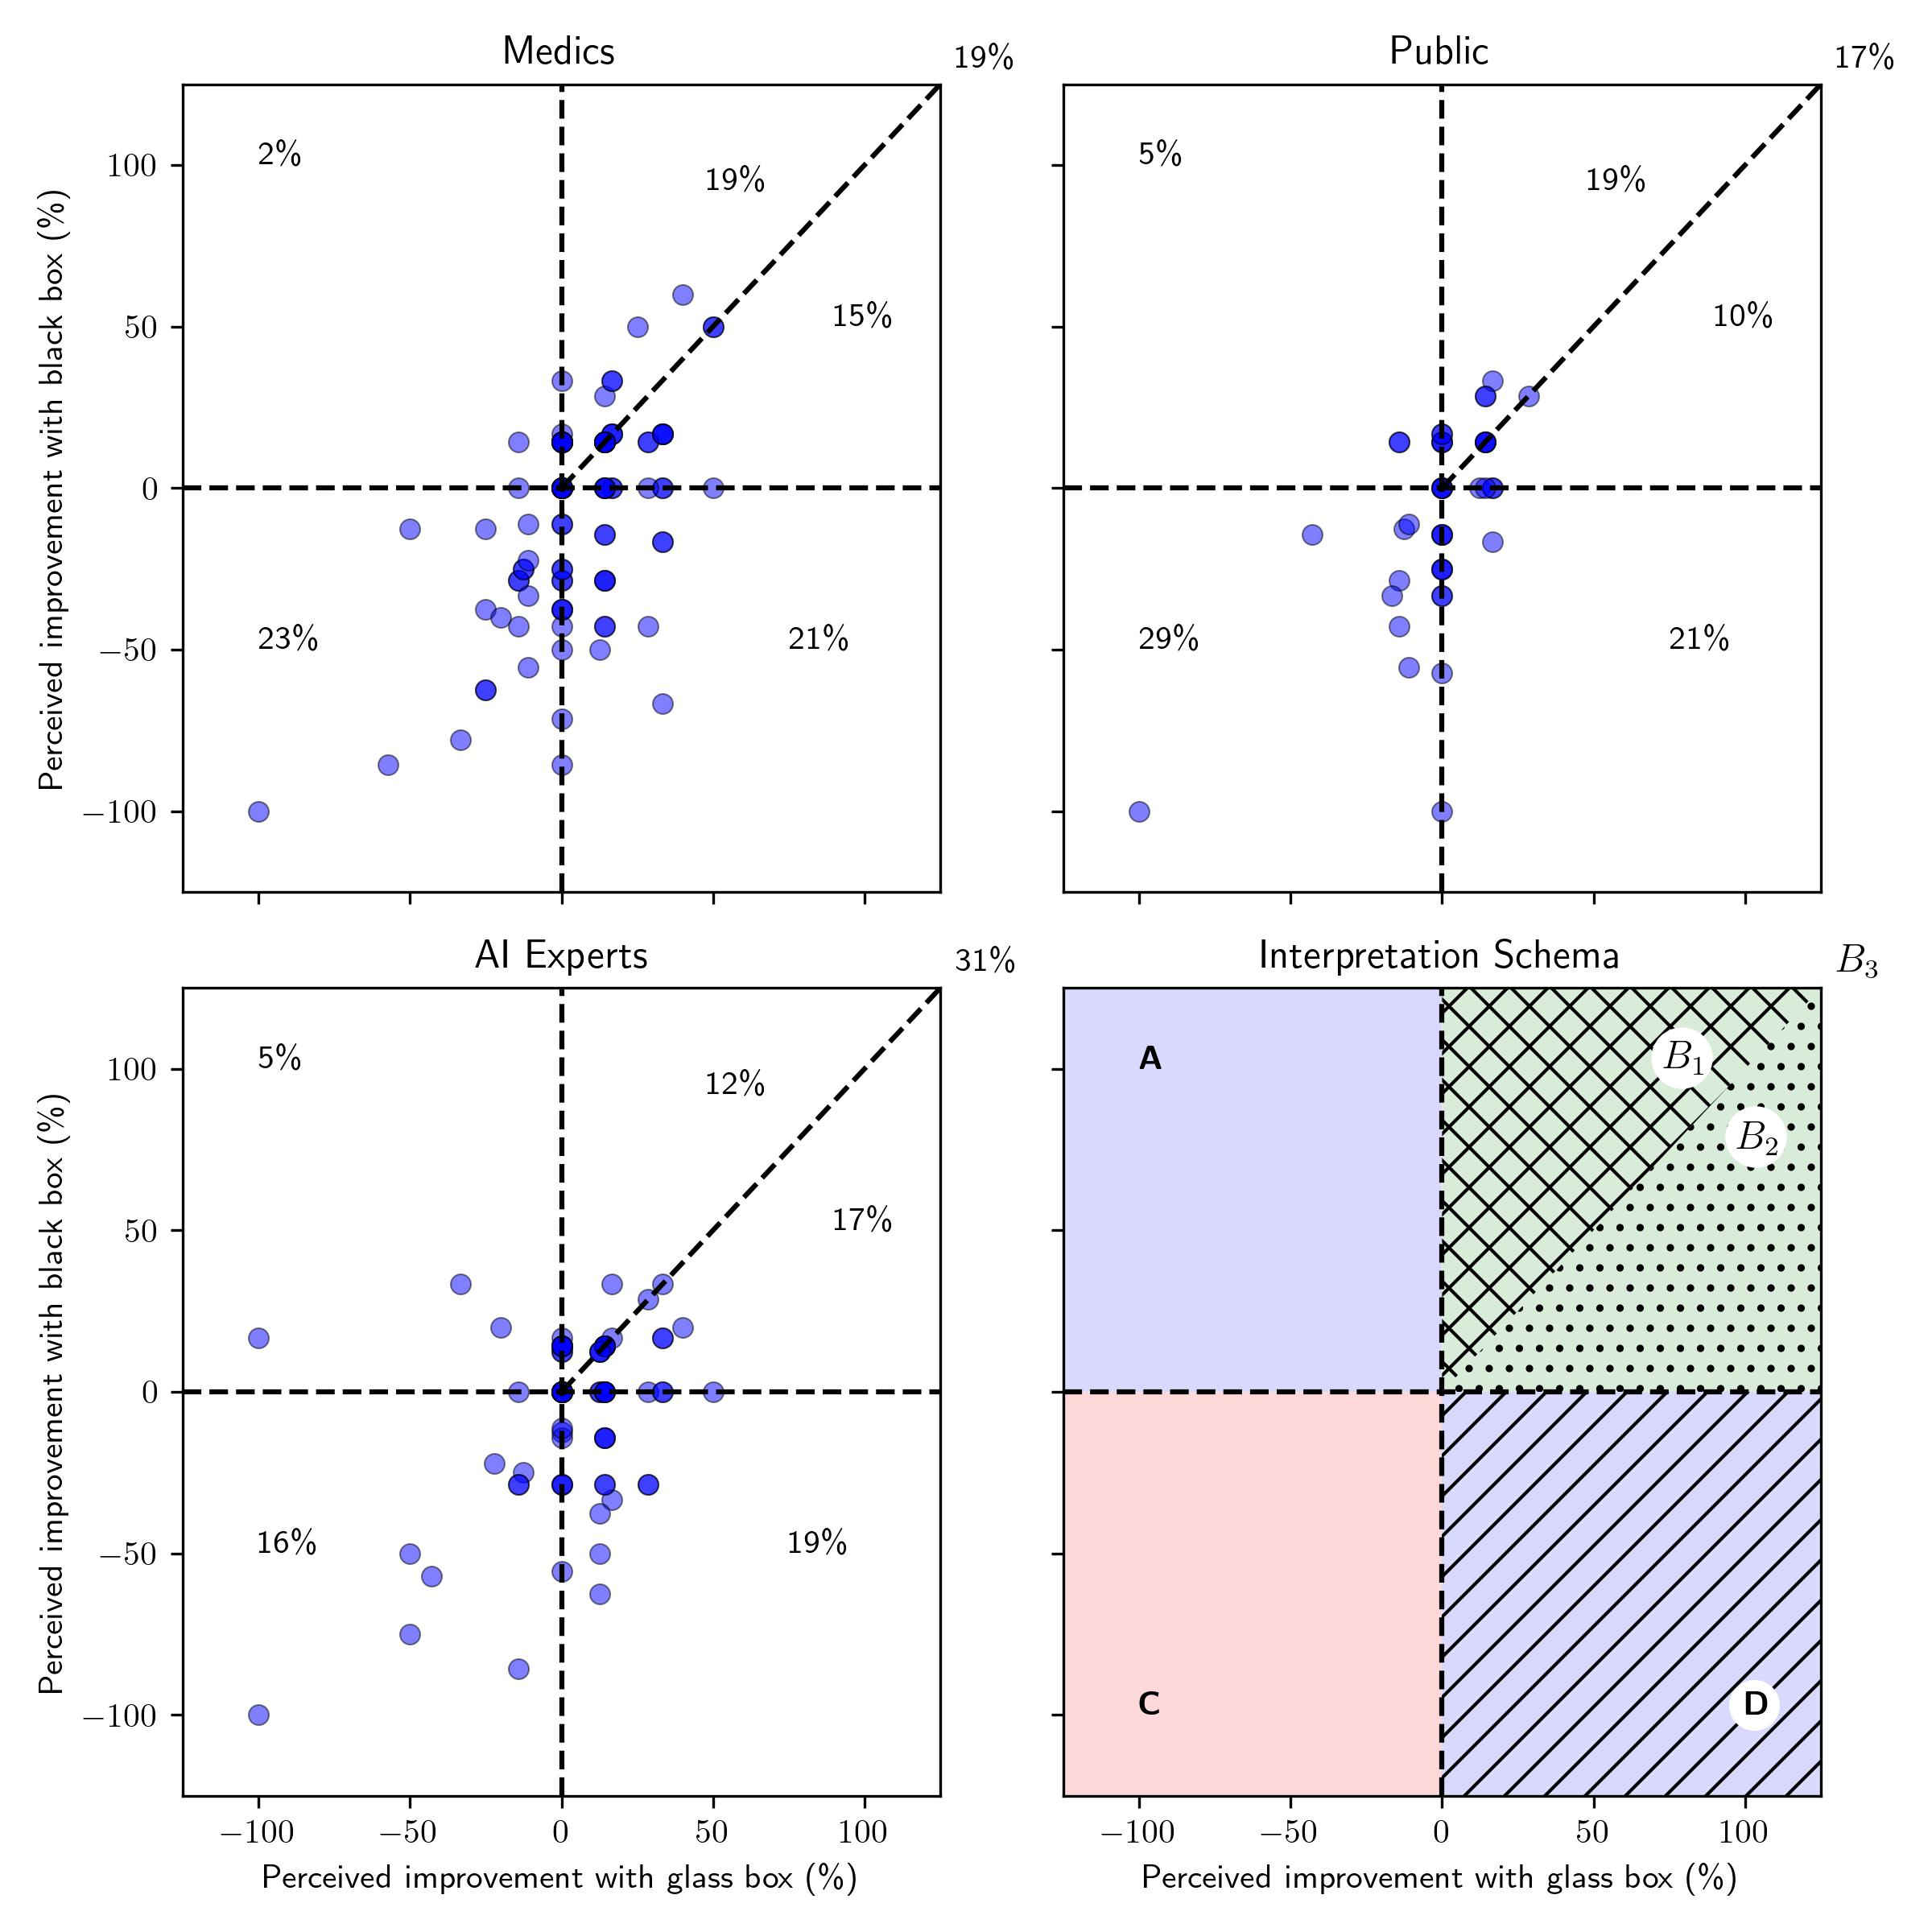
\includegraphics[width=\textwidth]{graphics/Doctor_improvements_cooperation_scatter.jpg}
    \caption{\centering Perceived improvements in trust in scenarios 3 and 4. Gaussian Kernel Density Estimates of the samples are included for visualisation clarity. Percentages are calculated using $\leq 0$ and $>0$ basis.\hspace{\textwidth} Interpretation schema: \textbf{A}: Black box improves diagnosis, glass box makes diagnosis worse \hspace{\textwidth} \textbf{B}: Both glass box and black box improve diagnosis. \textbf{$B_1$} black box is preferred, \textbf{$B_2$} glass box is preferred, $B_3$ neither is preferred. \textbf{C}: Neither glass box nor black box improve diagnosis \textbf{D}: Glass box improves diagnosis, black box makes diagnosis worse}
    \label{fig:improvement}
\end{figure}

Through Figure \ref{fig:improvement} we derive how different cohorts view the use of AI in cooperative scenarios. In all cohorts, a significant proportion of participants view the use of AI as beneficial with both models - 46\% of the public, 53\% of medical professionals, and 60\% of AI experts. This can be assumed to match the progression of technical expertise between cohorts.

Only a minority of each cohort view neither AI-cooperative scenario as beneficial. In all cohorts the glass box model is preferred over the black box model, but only by a small margin, with ratios $f_{BB}:f_{GB}$ of 1:1.17, 1:1.125 and 1:1.40 for the public, medical professionals and AI experts respectively. 

%\subsection{Correlation Analysis}

\subsection{Clustering}

Having disaggregated into profiling features, then analysed the trust levels of these cohorts, we can instead do the opposite. By starting with trust levels and finding distinct groups of how they are distributed, we can construct cohorts based on trust levels, then use profiling features to find the characteristics of these groups.

Insights can be gained into the results of the survey by applying unsupervised methods. These do not rely on any labels or targets, as would be the case in supervised or semi-supervised methods, so avoid many of the biases that such methods would carry. In particular we apply Uniform Manifold Approximation and Projection (UMAP) \cite{McInnes2018} as dimensionality reduction, then Hierachical Density-Based Spatial Clustering And Noise (HDBSCAN) \cite{McInnes2017} as unsupervised clustering on the resulting UMAP embedding. 

UMAP makes the assumption that data is distributed on a uniform manifold, but that the data-space is warped. Using this assumption local distance metrics are learnt, then used to construct a distance graph of the data. A lower-dimensional embedding is then formed, which aims to conserve the form of the high-dimensional space, using a stochastic graph layout. HDBSCAN, similarly, constructs a minimum spanning tree based on distances in the data-space, then applies various sub-algorithms to find clusters. Full explanation of these algorithms is beyond the scope of this work, so the reader should consult the relevant papers for more information.

We apply UMAP, then HDBSCAN to the resulting embedding, and present the results in Figures \ref{fig:embedding}, \ref{fig:cluster_means}. UMAP produces four distinct clusters, which are recognised by HDBSCAN. 

\begin{figure}
\centering
\begin{subfigure}{0.5\textwidth}
  \centering
  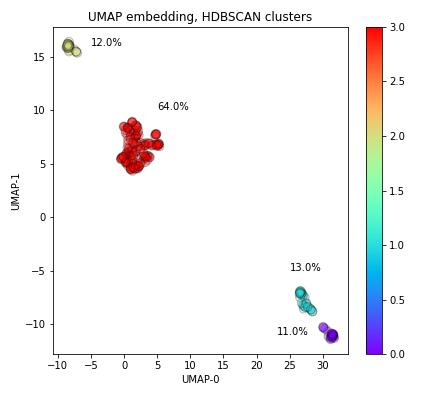
\includegraphics[width=\linewidth]{graphics/UMAP_HDBSCAN.jpg}
  \caption{}
%   \caption{The UMAP embedding produces four (visually) distinct clusters, which are also identified by HDBSCAN.}
  \label{fig:embedding}
\end{subfigure}%
\begin{subfigure}{0.55\textwidth}
  \centering
  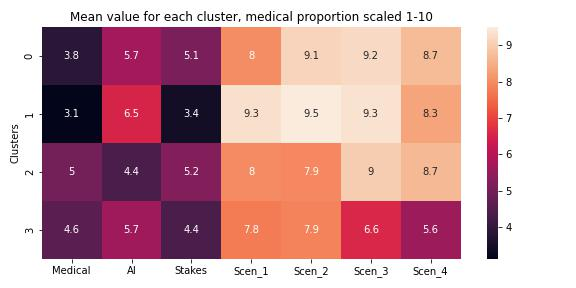
\includegraphics[width=\linewidth]{graphics/clustering_means.jpg}
  \caption{Cluster means across all four scenarios, along with profiling features.}
  \label{fig:cluster_means}
\end{subfigure}
\caption{The results of unsupervised clustering with UMAP and HDBSCAN. In Figure \ref{fig:cluster_means} profile features (AI, Medical, Stakes) are normalised by the whole population. Scenario trust levels are moved to a scale [0-1] for greater clarity in the heatmapping.}
\label{fig:test}
\end{figure}

The clusters identified by this process are distinct in how the participants within them rated trust in the different scenarios. Clusters 1 and 3 follow the same trend, with the highest trust in the glass-box cooperative scenario, and lowest in the solo black-box. However, cluster 3 has significantly lower trusts across all scenarios. Cluster 3 is significantly larger than the other clusters, representing 64\% of the participant pool.

Clusters 0 and 2 have the lowest level of trust placed in the doctor, with the solo black-box scenario scoring higher, in contrast to the opposite relationship in clusters 1 and 3. In both cluster 0 and 2 the highest trust is in the black-box cooperative scenario. Cluster 2 is the only cluster in which the glass-box cooperative scores lower than the solo doctor.

This analysis of only prescribed trusts leads to an intuitive split: In evaluating the compromise between transparency and efficacy, those in clusters 0 and 2 prescribe more weight to efficacy, and those in clusters 1 and 3 weight transparency over efficacy. Those in cluster 0 are perhaps closer to even balancing of transparency and efficacy than those in cluster 2, as shown by their higher trust levels in the glass-box scenario.

Cluster 1 probably represents our population of AI researchers - high average AI knowledge, but low stakes decision making and a small medical proportion. These participants rate any doctor-lead scenario highly, and only show a significant decrease in trust when a doctor is not presented as making the final decision, as in scenario 4.

Cluster 2, which leans the most towards following efficacy statistics, has the highest proportion of both medics and high-stakes decision makers. This might indicate that the cluster is composed principally of medical professionals, who are likely to rate themselves as more frequently making high-stakes decisions. This would also explain why this cluster has the lowest average self-reported AI knowledge compared to the whole survey population.

Clusters 0 and 3 are less easily identified, but might represent different subsets of the general population. Cluster 0 has a higher self-reported stake level, but a lower than average medic proportion, so might represent high-stakes decision makers from outside the medical field. Cluster 3 is very close to the average in all three of our profiling features, and is the largest, so could be said to represent the public, or the equivalent for our participant pool.

\subsection{Notes on results for discussions:}

\subsubsection{Cooperation:}
\begin{itemize}
    \item AI experts like the AI cooperation scenarios most - 60\% have higher trust than in doctor
    \item If you like the black box, you also like the glass box, and very few in any population only like the black box
    \item AI experts have the smallest proportion liking the glass box and disliking the black box
    \item Disliking both glass box and black box follows AI technical level: Public $\rightarrow$ Medics $\rightarrow$ AI
\end{itemize}

\subsubsection{Clustering:}
\begin{itemize}
    \item Clustering isolates medics and AI researchers
    \item AI researchers follow what we'd expect: they trust AI the most, but weight towards transparency over efficacy, and don't like the black-box working solo
    \item Medics weight heavily towards efficacy, but still rate a doctor having the final decision higher than the black box by itself
    \item General population is split into low/high stakes
    \item High-stakes genpop are less scared of AI, and seem to weight efficacy and transparency equally important, but still want a human final decision
    \item Low-stakes genpop (the actual public?) are scared of AI, especially when its not transparent. They don't like the Terminator doctor, sorry Arnold.
\end{itemize}






\subsection{Brainstorm}
\begin{itemize}
    \item Correlation analysis
    \item Clustering analysis
\end{itemize}




\subsection{Bit of maths}

In order for the AI to have any impact on the doctor, the doctor has to actually take the AI's diagnosis into account. For an AI diagnosis $A^x, x\in \{+,- \}$ and an original doctor diagnosis $D^x, x\in \{+,- \}$. As shown visually in Fig. \ref{fig:coop_diagram}, we can model a bias factor $f^x_{\textrm{Agree/Disagree}}$. The doctor can be assumed to carry a unique bias towards agreeing or disagreeing with the AI, dependent on the AI's diagnosis, which here we've modelled as a factor change to the doctor's original efficacy.

\tikzstyle{arrow} = [thick,->,>=stealth]
\tikzstyle{node} = [rectangle, text centered, draw = black, fill = white!255, minimum width = 2.5cm]
\tikzstyle{correct} = [rectangle, text centered, draw = black, fill = green!50, minimum width = 2.5cm]
\tikzstyle{incorrect} = [rectangle, text centered, draw = black, fill = red!30, minimum width = 2.5cm]

\begin{figure}[h]
\centering

\begin{tikzpicture}[node distance=2cm]
\node (patient) [node] {Patient symptoms};

\node (AI_pos)  [node, right of = patient, xshift = 2cm] {AI positive diagnosis};
\node (AI_neg)  [node, below of = patient, yshift = -0cm] {AI negative diagnosis};

\node (Pos_pos) [correct, right of = AI_pos, xshift = 4cm] {Doctor agrees, positive diagnosis};
\node (Pos_neg) [incorrect, above of = AI_pos, yshift = 0cm] {Doctor disagrees, negative diagnosis};

\node (Neg_pos) [incorrect, right of = AI_neg, xshift = 5cm] {Doctor agrees, negative diagnosis};
\node (Neg_neg) [correct, below of = AI_neg, yshift = -0cm] {Doctor disagrees, positive diagnosis};

\draw [arrow] (patient) -- node[anchor=south] {$A^+$} (AI_pos);
\draw [arrow] (patient) -- node[anchor=west] {$A^-$} (AI_neg);

\draw [arrow] (AI_pos) -- node[anchor=south] {$f^+_{\textrm{Agree}}D^+$} (Pos_pos);
\draw [arrow] (AI_pos) -- node[anchor=west] {$f^+_{\textrm{Disagree}}D^-$} (Pos_neg);

\draw [arrow] (AI_neg) -- node[anchor=south] {$f^-_{\textrm{Disagree}}D^+$} (Neg_pos);
\draw [arrow] (AI_neg) -- node[anchor=west] {$f^-_{\textrm{Agree}}D^-$} (Neg_neg);

\end{tikzpicture}

\caption{The process of AI-cooperative diagnosis}
\label{fig:coop_diagram}
\end{figure}

In this model the probability of a correct diagnosis for a patient with COVID is:

\begin{equation}
    P(\textrm{correct}) = (f^+_{\textrm{A}}A^+ + f^-_{\textrm{D}}A^-) D^+
\label{eqn:correct_coop}
\end{equation}

with $f^+_{\textrm{A}}$ shorthand for $f^+_{\textrm{Agree}}$, and the same shortening notation for $f^-_{\textrm{Disagree}}$. We can assume that the probability of a correct diagnosis is limited to $0 \leq P(\textrm{correct}) \leq 1$, which sets limits

\begin{equation}
    0 \leq f^+_{\textrm{A}}A^+, f^+_{\textrm{D}}A^- \leq 1/D^+
\end{equation}


In this model the patients diagnosis is only improved if $(f^+_{\textrm{A}}A^+ + f^-_{\textrm{D}}A^-) > 1$, otherwise the chance of a COVID positive patient being correctly diagnosed decreases. Important to note is that if $f^+_A \textrm{ and } f^-_D = 1$, ie if the doctor has no interpretation of the AI's diagnosis, then Equation \ref{eqn:correct_coop} becomes

\begin{equation}
    P(\textrm{correct}) = (A^+ + A^-) D^+ = D^+
\end{equation}

the effect of which being that the AI has no impact on the doctor's efficacy. 


% \begin{figure}[h]
% \centering

% \begin{tikzpicture}

% \draw[opacity=0.5,fill=green!50] (0pt, 6cm) -- (0pt, 9cm) -- (9cm, 0pt) -- (6cm, 0pt) -- (0pt, 6cm);
% \draw[opacity=0.5,fill=red!30] (0pt, 0pt) -- (0pt, 6cm) -- (6cm, 0pt) -- (0pt, 0pt);

% \draw[thick,->] (0,0) -- (10,0) node[anchor=north west] {$f^+_{\textrm{A}}A^+$};
% \draw[thick,->] (0,0) -- (0,10) node[anchor=south east] {$f^-_{\textrm{D}}A^-$};

% \draw (9cm,2pt) -- (9cm,-2pt) node[anchor=north] {$1/D^+$};
% \draw (2pt, 9cm) -- (-2pt, 9cm) node[anchor=east] {$1/D^+$};
% \draw (0pt, 9cm) -- (4.5cm, 4.5cm) node[anchor=west] {Upper probability limits};
% \draw (4.5cm, 4.5cm) -- (9cm, 0pt) node[anchor=west] {};

% \draw (6cm,2pt) -- (6cm,-2pt) node[anchor=north] {$1; f^+_A = 1/A^+$};
% \draw (2pt, 6cm) -- (-2pt, 6cm) node[anchor=east] {$1; f^-_D = 1/A^-$};
% \draw (0pt, 6cm) -- (3cm, 3cm) node[anchor=west] {Improved diagnosis};
% \draw (3cm, 3cm) -- (6cm, 0pt) node[anchor=west] {};

% \draw [dotted] (4.5cm, 1pt) -- (4.5cm, 1.5cm); 
% \draw [dotted] (4.5cm, 1.5cm) -- (1pt, 1.5cm); 
% \draw (4.5cm,0pt) -- (4.5cm,-2pt) node[anchor=north] {$A^+$};
% \draw (0pt,1.5cm) -- (-2pt, 1.5cm) node[anchor=east] {$A^-$};

% \draw [dashed] (3cm, 1pt) -- (3cm, 3cm); 
% \draw [dashed] (3cm, 3cm) -- (1pt, 3cm); 
% \draw (3cm,0pt) -- (3cm,-2pt) node[anchor=north] {$D^+$};
% \draw (0pt,3cm) -- (-2pt, 3cm) node[anchor=east] {$D^-$};

% \draw (1pt,1pt) -- (-1pt, -1pt) node[anchor=north east] {$0,0$};

% \end{tikzpicture}

% \caption{\centering Regions of diagnosis efficacy in a human-AI cooperative scenario, with $f^{+/-}_{A/D}$ bias factors when interpreting the AI diagnosis $A^{+/-}$, and the non-AI doctor diagnosis $D^{+/-}$. Not to scale with the values in the survey scenarios.}
% \label{fig:my_label}
% \end{figure}

% \begin{figure}[h]
% \centering

% \begin{tikzpicture}

% \draw[opacity=0.5,fill=red!50] (0cm, 4cm) -- (4cm, 4cm) -- (4cm, 0cm) -- (0cm, 0cm) -- (0cm, 4cm);

% \draw[opacity=0.5,fill=blue!30] (0cm, 4cm) -- (0cm, 6cm) -- (4cm, 6cm) -- (4cm, 4cm) -- (0cm, 4cm);

% \draw[opacity=0.5,fill=green!30] (4cm, 4cm) -- (4cm, 6cm) -- (6cm, 6cm) -- (6cm, 4cm) -- (4cm, 4cm);

% \draw[pattern=north west lines, pattern color=blue!30, opacity=0.5] (4cm, 0cm) -- (4cm, 4cm) -- (6cm, 4cm) -- (6cm, 0cm) -- (4cm, 0cm);

% \draw (2cm,5cm) -- (2cm,5cm) node[anchor=north] {A};
% \draw (5cm,5cm) -- (5cm,5cm) node[anchor=north] {B};
% \draw (2cm,2cm) -- (2cm,2cm) node[anchor=north] {C};
% \draw (5cm,2cm) -- (5cm,2cm) node[anchor=north] {D};

% \draw (3cm,0pt) -- (3cm,0pt) node[anchor=north] {Glass box trust factor change};
% \draw (0pt,3cm) -- (0pt,3cm) node[anchor=east, rotate=-90, xshift=2cm, yshift=-7pt]  {Black box trust factor change};

% \end{tikzpicture}

% \caption{\centering Interpretation schema for cooperative improvement plots. \textbf{A}: Black box improves diagnosis, glass box makes diagnosis worse \textbf{B}: Both glass box and black box improve diagnosis \textbf{C}: Neither glass box or black box improve diagnosis \textbf{D}: Glass box improves diagnosis, black box makes diagnosis worse}
% \label{fig:quadrant explanation}
% \end{figure}



From this model we can define some doctor profiles based on how they might interact with an AI tool:

\begin{itemize}
    \item \textbf{$f^+_A, f^-_D = 1/D^+$:}  A doctor who trusts the AI's positive diagnoses completely, but also catches every single mis-classification by the AI
    \item \textbf{$f^+_A, f^-_D = 0$:}      A doctor who never agrees with a positive AI diagnosis, and always agrees with a negative AI diagnosis
    \item ETC, FLESH OUT LATER
\end{itemize}

\subsection{Focus Group}
\begin{itemize}
    \item Goals, how does it follow from survey data? (does trust mean you will be happy to use the AI?)
    \item Who do we want to talk to? How will we use the information?
    \item 
\end{itemize}

A focus group study was devised as a follow-up to the survey study, to gain insight into the reasoning and motivation behind survey responses, and to uncover topics of interest and concern as well as differences in opinion surrounding AI decision support tools.  



\subsubsection{Recruitment}

Recruitment was performed via the survey from Section [link to section?] - participants were presented with an option to provide an email address if they were interested in being contacted to participate in the focus group. Following the collection and analysis of survey data, a recruitment survey was sent to the participants of the first survey who agreed to be contacted. The recruitment survey was designed to gather a small amount of demographic information so that an appropriate spread of participants were included [change wording].

[What is the requested demographic information? Use questionnaire data or ask for more? Inclusion of BAME and gender?]

Subreddits:
\begin{itemize}
    \item r/machinelearning
    \item r/london - awaiting approval
    \item r/coronavirusuk - awaiting approval
\end{itemize}

This demographic information was used to recruit at least one person from the following categories:

\textbf{Category 1: Experienced Senior AI Expert}
\begin{itemize}
\item High self-reported rating in AI expertise.
\item Not a medical professional.
\item Mid to high self-reported involvement in high-stakes decision making
\end{itemize}
(Ideally in a senior role or management position).

\textbf{Category 2: AI Specialist}
\begin{itemize}
\item Mid to high self-reported rating in AI expertise.
\item Not a medical professional.
\item Low self-reported involvement/responsibility in high-stakes decision making.
\end{itemize}

Ideally not in a senior role or management position, could be early career or still in education)

\textbf{Category 3: Experienced Senior Healthcare Expert}
\begin{itemize}
\item Low to Mid self-reported rating in AI expertise
\item Is a medical professional, 
\item High self-reported involvement/responsibility in high-stakes decision making
\end{itemize}

Ideally in a senior role or management position in a clinical hospital setting.

\textbf{Category 4: Healthcare Specialist}
\begin{itemize}
\item Low self-reported rating in AI expertise
\item Is a medical professional.
\item Mid to High self-reported involvement/responsibility in high-stakes decision making
\end{itemize}

Ideally in a role with some responsibility for high-stakes decision making, or a role in which they provide information and evidence which supports others in making high stakes decisions. 

This individual should be employed in a clinical hospital setting (could still be in education and training, but should currently be undertaking practical rotations, or have practical responsibilities in a clinical hospital setting). 


\textbf{Category 5: Wildcard}
Any combination of self-reported traits.
Could be a member of the public.
Could be a second member of any previous category. 
Possibility of being a clinical informatician, or other clinical computer scientist.
Possibility of being a software engineer who has experience with developing medical devices. 

[Explain why you wanted to recruit people at the end of each spectrum, and avoid people who cross the demographics]

\subsubsection{Topics of Discussion}



\subsubsection{Data Gathering and Analysis}
Interviews were conducted via Microsoft Teams [University of Bristol server?]. The audio from the entire session was recorded, and stored temporarily on a secure server. The session audio was used create an anonymised transcript, then promptly deleted. 

Thematic analysis was performed on the focus group transcript using NVivo [cite]. 

[Describe how you will do thematic analysis on the focus group data].




\subsubsection{Results}
A single focus group comprising five participants was held in April 2022.

\section{Design}


\section{Findings}
Describe our findings from user research
Evaluation of our findings

\section{Discussion}
Contribution we've made


\section{Conclusion}



%%
%% The acknowledgments section is defined using the "acks" environment
%% (and NOT an unnumbered section). This ensures the proper
%% identification of the section in the article metadata, and the
%% consistent spelling of the heading.
\begin{acks}
Acknowledgments
\end{acks}

%%
%% The next two lines define the bibliography style to be used, and
%% the bibliography file.
\newpage
\bibliographystyle{ACM-Reference-Format}
\bibliography{elf}

%%
%% If your work has an appendix, this is the place to put it.
\appendix

\section{Optional Supplementary Material}

\subsection{Study Ethics}

% DC - Need to go through and format, I've been working in a google doc
% How do I add line space after subsubheading?
\subsubsection{Organisation and Funding}


This work was organised and funded by The University of Bristol School of Computer Science, Electrical and Electronic Engineering, and Engineering Maths.

Investigators are students enrolled on the “Interactive Artificial Intelligence CDT” at the University of Bristol, and are funded by UKRI Studentships.

This work was completed as part of a University course “Interaction Design COMSM0087”, led by Dr Paul Marshall.


\subsubsection{Ethical Approval} 


Ethical approval for study methods described in Section [?] of the report was granted by University of Bristol Faculty of Engineering Research Ethics committee prior to study recruitment.

The study has been reviewed by the unit director, Dr Paul Marshall.

The risks associated with participating in the study were assessed as low likelihood and low severity. 

\subsubsection{Incentive}  


At the recruitment stage, prospective participants were told that there would be a monetary incentive for participation.

For participation in the survey, this was the option to be entered into a raffle to win one of four Amazon gift vouchers worth £25 each.

To facilitate this, participants could opt in to the raffle by providing an email address, which was stored securely on a University server. 

Email addresses were stored separately from survey responses to prevent any reassociated. 

At the time that the survey was closed to new participants, four email addresses were selected at random to receive the vouchers.

Once the selected participants had confirmed they received the vouchers, all email addresses were promptly deleted. 



\subsubsection{Privacy and Data Management}  


Survey:
No personal identifiable information was collected during the survey phase of this work.

Survey data was collected via Microsoft Forms, and stored on a secure server hosted by the University of Bristol.

Participants had the option of providing an email address to opt into a raffle to win a monetary prize. 
This email address was not associated with their survey response, and was used only to send the prize to the relevant participants. 
Email addresses were stored on a secure University of Bristol server and deleted after prizes were allocated.  

Focus Group:
The focus-group was conducted remotely via Zoom online video conferencing. 

The focus-group was recorded for the purpose of transcribing the discussion, and was deleted when the audio had been transcribed. 

All audio transcriptions were pseudonymised prior to analysis.

All data gathered for this work (survey responses, email addresses, focus-group audio, transcript) was stored on a secure University of Bristol server. 

\subsubsection{Recruitment:}  


The total number of survey participants was [XXXX] at the time of closing.
Survey participants were recruited by:
Direct contact
Sharing the survey with personal contacts
Mailbases 
Survey was sent to the directors of the following University programs to be  distributed to the students:
[Which programmes?]
The survey was posted in a medical physics and engineering special interest mailing group: JISCMAIL Medical-Physics-Engineering 
Social media
The survey was distributed through personal Twitter accounts.
Participation was open to all members of the public, however recruitment was targeted towards three groups: healthcare professionals, AI/ML specialists, and general public. The studies population is not therefore reflective of a cross-section of the general public or specific demographic groups. 
No demographic information relating to protected characteristics was collected. 
The only objective information requested from participants was whether or not they work as a healthcare professional. 
Six focus-group participants were recruited from personal contacts. 

\subsubsection{Informed Consent Survey}  


Written consent was obtained for the survey study…
A participant information sheet was presented at the start of the survey. Participants were required to confirm that they have read the information sheet before progressing with the survey to ensure informed consent as much as was reasonably practicable. 
I.e. “By clicking "Next" you confirm that you've read the full information about this study and consent to participate.”
The participant information sheet included:
Background about the project and project organisers.
The purpose of the study
Reason participants have been recruited. 
Eligibility criteria
Details of participation:
Emphasis that participation is voluntary
Emphasis that participant can choose to withdraw from the study (relevant to focus group).
Description of how data will be managed and used.
Details of incentive.
Details of confidentiality. 
Emphasis that no personally identifiable information is recorded in the survey. 
Right to withdrawal.
Contact details for asking questions. 
Intended outcomes of the research project.
Eligibility criteria i.e. requirements for participation as specified in the information sheet include:
Participant is over 18 years old
Participant has internet access to participate in online data collection

 
\subsubsection{Informed Consent Focus-Group}  


Participants were sent an information sheet directly, and asked to confirm they had read and understood the provided information prior to the event.

At the start of the focus group session, participants were given the opportunity to say if they had not read or understood the provided information, or if they had any concerns they wanted to raise. 

\subsubsection{Other}  



%Check notes from other group
%Check any other comments/document related to ethics
%So far, I've mostly just looked at the ethical approval document and the details from our information sheet.


% DC - Need to go through and format, I've been working in a google doc
% How do I add line space after subsubheading?


\subsection{Part Two}  




\end{document}
\endinput
%%
%% End of file.
